\section{Analysis overview}\label{section:heavyflavour}
Measurements of electrons from heavy-flavour hadron decays are  obtained selecting an inclusive electrons sample and subtracting the electrons which do not originate from heavy-flavour hadron decays. The measurements were performed by identifying electrons after combining two different  strategies with different detectors offering the largest $p_{\rm{T}}$ reachable. In particular, it ensures that the systematic uncertainties and the hadron contamination are small over the whole transverse momentum range. Electron identification is performed using the TPC and TOF detectors in the momentum range $0.2 < p_{\rm{T}} < 4$ GeV/$c$. The requirement of TOF in this momentum range improves the rejection of hadronic background. At higher $p_{\rm{T}}$ (from 3 \GeVc), electron identification was based on the combined information from the TPC and the EMCal detectors. 
Throughout the paper, the term ‘electron’ is used for electrons and positrons. 



\subsection{Electron identification}
Reconstructed tracks were selected based on the criteria listed in Table~\ref{Table:InclusiveTrackSelection}, which are similar to those used in the analysis described in ~\cite{Acharya:2019hao, Acharya:2019mom}. These requirements are applied depending on the data sample as well as the transverse momentum region of the analysis. %In the analysis of {\color{cyan}pp collisions with low }{\color{purple} and nominal magnetic field} and p-Pb data sample, the cut on the minimum number of ITS clusters was reduced to {\color{cyan}three} \sout{(instead of four used in pp collisions {\color{cyan} with normal magnetic field})} because the SDD points, which were not available, were excluded from the track reconstruction used for this analysis, thus limiting the maximum number of hits in the ITS to {\color{purple}three}.  
In order to reduce wrong assignations of hits in the first layer of the SPD to the candidate tracks and to reduce the background from photon conversions in the material, hits in both layers of the SPD
were required in the TPC--TOF analysis. In the TPC--EMCal analysis, this requirement has been relaxed to at least one hit in any of the two SPD layers in order to increase the statistics. 

\begin{table}[h!]
\caption{Summary of the track selection criteria imposed on the inclusive electron candidates for different datasets and different detectors.} \\
\centering
\small
\begin{tabular}{c|ccc|cc}
\hline\hline
 & \multicolumn{3}{c|}{pp 13 TeV} & \multicolumn{2}{c}{p--Pb 8.16 TeV}  \\ 
 Track selection & Low B & Nominal B  & Nominal B & Nominal B & Nominal B \\
  criteria & TPC--TOF & TPC--TOF  & TPC--EMCal & TPC--TOF & TPC--EMCal \\

%Track selection & \multicolumn{3}{c|}{pp 13 TeV} & \multicolumn{2}{c}{p--Pb 8 TeV}  \\ 
%criteria & $p_{\rm T}$ $<$ 0.5 & 0.5 $<$ $p_{\rm T}$ $<$ 3 & $p_{\rm T}$ $> 3$ &  $p_{\rm T} < 3 &  $p_{\rm T}$ $>$ 3 \\ [0.5ex] 
 %& (\GeVc) & (\GeVc) & (\GeVc) &  (\GeVc) &  (\GeVc)\\ [0.5ex]
\hline 
%$p_{T}^{min}$ &  0.5 GeV/c &  0.5 GeV/c& 0.0 GeV/c \\
$|\eta|$ & $<$ 0.5 & $<$ 0.8 & $<$ {0.7} & $<$ 0.8 & $<$ 0.6 \\
{No. of TPC } & $\geq$ 70 & $\geq$ 70  &  $\geq$  70   & $\geq$ 70  & $\geq$ 70   \\
CrossedRows &  &  &   &   & \\
No. of TPC d$E$/d$x$& $\geq$ 80 & $\geq$ 80 &  $\geq$ {80} & $\geq$ 80 & $\geq$ 80\\
 clusters for PID &  &  & &\\
Number of ITS hits & $\geq$ {3} & $\geq$ {3}& $\geq$ {3} & $\geq$ 3& $\geq$ 3\\

%\item Ratio found / findable TPC clusters $>$ 0.6
$\chi^{2}$ /clusters of & $<$ 4 & $<$ 4 & $<$ 4 &$<$ 4&$<$ 4\\
momentum fit in TPC &  &  &&\\
%Ratio found / findable TPC clusters & $>$ 0.6 & $>$ 0.6 \\
% (\textcolor{red}{2})
Requirement of hits & kBoth & kBoth & kAny & kBoth & kAny\\%(\textbf{\textcolor{red}{kFirst}})
in SPD layers & & & & &\\
$|\rm DCA_{xy}|$ & $<$ 1 cm & $<$ 1 cm & $<$ 1 cm & $<$ 1 cm& $<$ 1 cm\\
$|\rm DCA_{z}|$ & $<$ 2 cm & $<$ 2 cm & $<$ 2 cm & $<$ 2 cm & $<$ 2 cm\\
%Kink mothers and daughters & excluded & excluded \\
%TOF $t$ - $<$ TOF $t>\mid _{el}$ in between & -3 to 3 $\sigma$ & -3 to 3 $\sigma$ & not used\\
%TPC $\frac{dE}{dX}$ - $<$ TPC $\frac{dE}{dX}>\mid _{el}$ in between  & -1 to 3 $\sigma$  & -1 to 3 $\sigma$ &  -3 to 3 $\sigma$\\
\hline
\end{tabular}
\label{Table:InclusiveTrackSelection}
\end{table}

To identify electrons with the TPC the specific energy deposition (d$E$/d$x$) in the detector was used. At low $p_{\rm T}$ $\leqslant$ 4 GeV/$c$,  the TOF detector was required to reduce background from kaons and protons. The discriminant  variable used for TPC (TOF) detector is the deviation of d$E$/d$x$ (particle time-of-flight) from the parameterised electron Bethe-Bloch (electron time-of-flight) expectation value~\cite{Bethe:1930ku}, expressed in terms of d$E$/d$x$ (time-of-flight) resolution, $n^{\rm{TPC}}_{\sigma,\rm{e}}$ ($n^{\rm{TOF}}_{\sigma,\rm{e}}$). In the left plot of Figure~\ref{fig:pp_13_TPCNsigma}, $n^{\rm{TPC}}_{\sigma,\rm{e}}$ as a function of momentum after TOF selection is shown.  At high $p_{\rm T}$ ($> 3$ GeV/$c$) the hadron contamination in the electron sample increases with transverse momentum, which is reduced using the EMCal detector. With the EMCal detector, electrons are identified and separated from hadrons using the $E/p$ information, where, $E$ is energy deposited by the particle in the detector and $p$ is momentum of the track.

In the analysis using TPC--TOF detectors, for $0.2 < p_{\rm T} < 4$ GeV/$c$, electron candidates are selected by requiring $|n^{\rm{TOF}}_{\sigma,\rm{e}}|$ $<$ 3 and -1 $<$ $n^{\rm{TPC}}_{\sigma,\rm{e}}$ $<$ 3, resulting in a 100\% pure electron sample at 0.2 \GeVc and decreases to 95\% purity at 4 \GeVc.
%electron sample with purity of {\color{cyan} about 100 -- 95$\%$ within range 0.2 $<$ $p_{\rm T}$ $<$ 4 GeV/c}. 
%The selection criteria of $n^{\rm{TPC}}_{\sigma,\rm{e}}$ allows a constant electron identification (eID) efficiency with the TPC of $\sim$86$\%$. 
The remaining hadron contamination in the sample, after TOF selection, is estimated and subtracted by parameterizing the TPC d$E$/d$x$ distribution for each particle species with an analytical function in different momentum regions as shown in the right plot of Figure~\ref{fig:pp_13_TPCNsigma} and done in previous analyses~\cite{Acharya:2019hao, Acharya:2019mom}. 

\begin{figure}[h!]
    %\centering
    \includegraphics[scale = 0.46]{figures/Results/HFE_pp_LowB/TPCQA_LowB.png}
    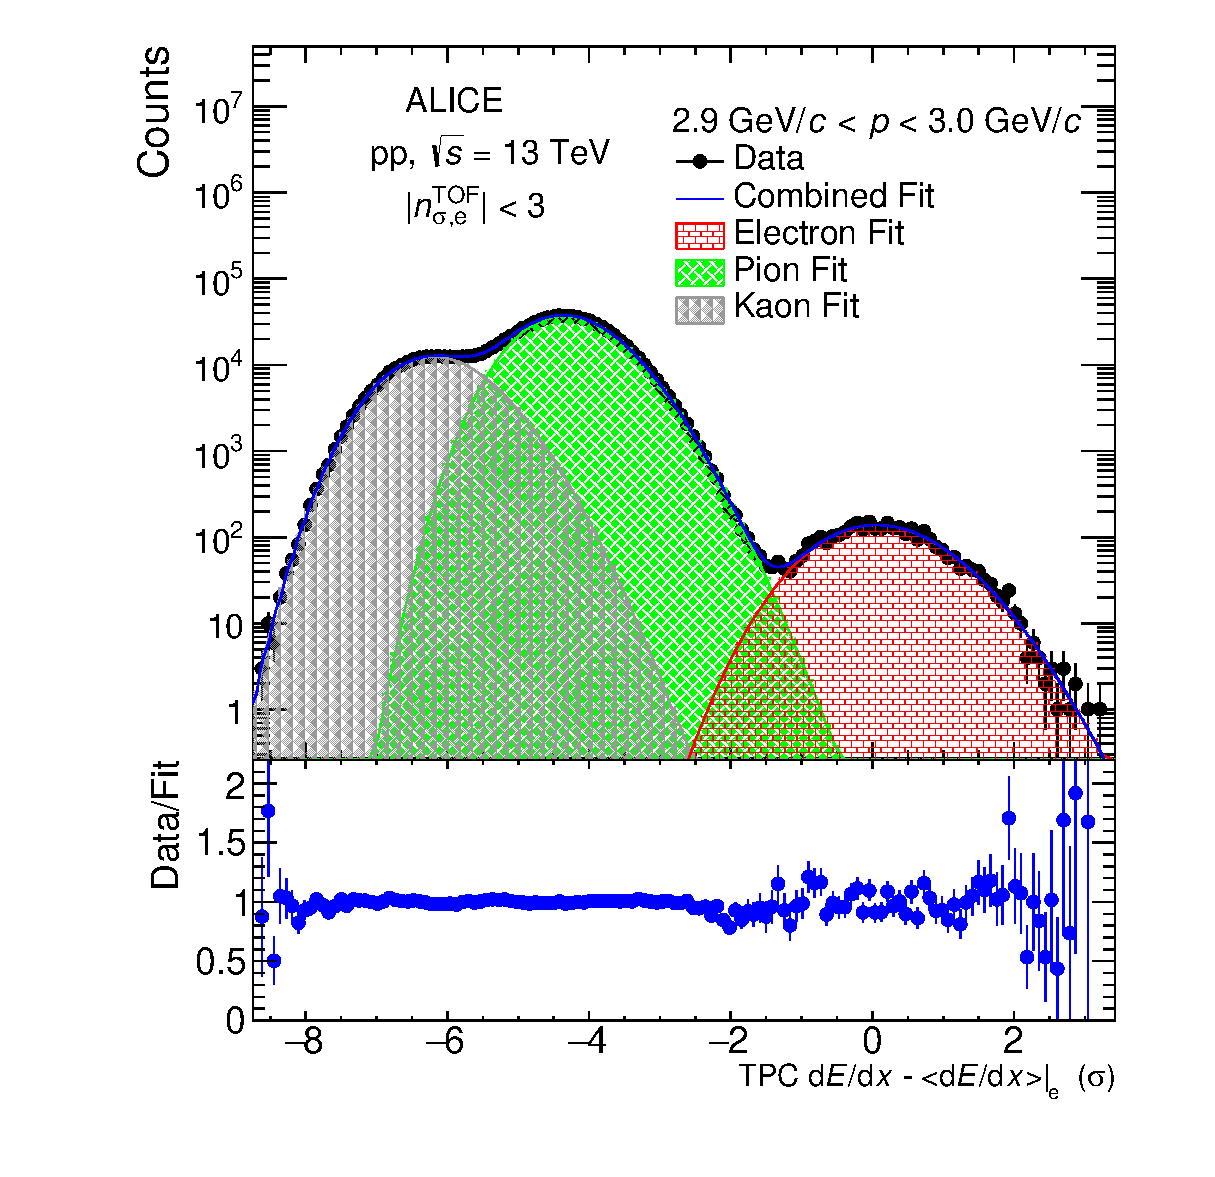
\includegraphics[scale = 0.35]{figures/Results/HFE_pp_LowB/TPCNsigma29to30_New.eps}
    \caption{TPC d$E$/d$x$ signal as a deviation from the expected electron energy loss after TOF selection (left) and Fit of $n^{\rm{TPC}}_{\sigma,\rm{e}}$ distributions of various species in pp collisions at $\sqrt{s}$ $=$ 13 TeV (right).} %{\color{blue} I see quite some issues here with the figure. we will for sure be asked why the kaon are not smooth in the right panel and why the fit at 0.2 GeV/c is not nice and what is the chi2 value we get. Don't we have better fit? Can the kaon be smoothened? Actually, do we need this figure at all (provocative ;))}}
    \label{fig:pp_13_TPCNsigma}
\end{figure}

 %In transverse momentum region 0.2 to 4 GeV/$c$, the particles are identified as electrons which satisfies the criteria of -1 $<$ $n^{TPC}_{\sigma,e}$ $<$ 3, which gives rise to the electron identification (eID) efficiency of 84$\%$. Moreover, the tracks with $|n^{TOF}_{\sigma,e}|$ $<$ 3, were accepted to overcome the ambiguities mentioned earlier. 
%The obtained electrons sample may still contain the contamination from the hadrons. The amount of this contamination is estimated by parameterizing the TPC d$E$/d$x$ distribution after TOF selection in different momentum regions for $p_{\rm T}$ $\leqslant$ 4 GeV/$c$, as done in previous analyses [ref]. 

In the analysis using TPC--EMCal detectors, for $p_{\rm T}$ $>$ 3 GeV/$c$, tracks with $-1 < n^{\rm{TPC}}_{\sigma,\rm{e}}$ $<$ 3 are selected. The electron sample was obtained by selecting candidates with $0.85 < E/p < 1.2$, as electrons are expected to be around unity, while hadrons have lower $E/p$ values. To further reduce the amount of hadron contamination, a condition on the shape of the electromagnetic shower ~\cite{Alessandro:2006yt}, $\sigma^{2}_{\rm{short}}$ and $\sigma_{\rm{long}}^{2}$, was
applied. $\sigma^{2}_{\rm{short}}$ and $\sigma_{\rm{long}}^{2}$ stands for the eigenvalues of the dispersion matrix of the shower shape ellipse defined by the energy distribution within the EMCal cluster ~\cite{Awes:1992yp, Acharya:2017hyu}. A \pt dependent selection of $0.02 < \sigma_{\rm{long}}^{2} < 0.9/0.7/0.5$ 
for $p_{\rm T} < 12 , 12- 20,  > 20$ GeV/$c$
in both pp collisions and in p-Pb collisions were chosen, as it reduces the hadron contamination while not significantly affecting the electron signal efficiency.  The lower threshold of $\sigma^{2}$ is chosen to remove contamination caused by neutrons hitting the readout electronics. The hadron contamination in the electron sample was estimated by measuring $E/p$ for hadrons with $n^{\rm{TPC}}_{\sigma,\rm{e}} < -3.5 $ for pp collisions  and $n^{\rm{TPC}}_{\sigma,\rm{e}} < -4$ for p-Pb collisions. The hadron $E/p$ distribution is scaled to match the electron candidate's $E/p$ distribution in the range $E/p<0.7$, as shown in Fig.~\ref{fig:pp_13_EbyP}. The electron yield was obtained by integrating the $E/p$ distribution for $0.85 < E/p < 1.2$. In pp (p-Pb) analysis, the hadron contamination was negligible at low $p_{\rm{T}}$, and increased to around $23\%$ ($25\%$) at $p_{\rm{T}} $ $=$ 35 (26) GeV/$c$, which was subtracted from the electron sample.

\begin{figure}[h!]
    \centering
    \includegraphics[height=6cm,width=7cm]{{figures/Results/HFE_ppNormalB/EbyP_MB}.pdf}
    \includegraphics[height=6cm,width=7cm]{{figures/Results/HFE_ppNormalB/EbyP_EG1}.pdf}
    \caption{E/p distribution for pp 13 TeV for MB (left) and EG1 (right) triggers}
    \label{fig:pp_13_EbyP}
\end{figure}

%\begin{table}[h]
%\caption{Summary of the particle identification criteria imposed on the inclusive electron candidates}
%\centering
%\begin{tabular}{c c c c c}
%\hline\hline
%Track and PID & pp 13 TeV  & pp 13 TeV & p--Pb 8 TeV & p--Pb 8 TeV\\ 
%cuts & $p_{\rm T}$ $\leqslant$ 4 GeV/$c$ & $p_{\rm T}$ $>$ 4 GeV/$c$ &  $p_{\rm T}$ $\leqslant$ 4 GeV/$c$ &  $p_{\rm T}$ $>$ 4 GeV/$c$\\ [0.5ex]
%\hline 
%TPC $\frac{dE}{dX}$ - $<$TPC$\frac{dE}{dX}>\mid _{el}$ & -1 to 3 $\sigma$  & -1 to 3 $\sigma$ &  0 to 3 $\sigma$ &  0 to 3 $\sigma$\\
%  &  &  &  &\\
%TOF $t$ - $<$TOF$t>\mid _{el}$ & -3 to 3 $\sigma$ & -- & -3 to 3 $\sigma$ & --\\
 %&  &  & &\\
%EMCal & -- &  & -- &  \\
% &  &  & &\\
%\hline
%\end{tabular}
%\label{Table:InclusivePIDSelection}
%\end{table}



\subsection{Subtraction of electrons from non heavy-flavour sources}
The selected inclusive electron sample contains electrons from open heavy-flavour hadron decays and from  different sources of background:

\begin{itemize}
    \item electrons coming from Dalitz decay of light-neutral mesons such as $\pi^{0}$, $\eta$ as well as conversion of photons in the detector material, termed as photonic electrons in the text. 
    \item di-electrons from J/$\psi$ (J/$\psi$ $\rightarrow$ $e^{+}e^{-}$) and low-mass vector mesons ($\rho$ $\rightarrow$ $e^{+}e^{-}$, $\omega$ $\rightarrow$ $e^{+}e^{-}$, $\phi$ $\rightarrow$ $e^{+}e^{-}$).
\item electrons from weak decays $\rm K^{0/\pm}$ $\rightarrow$ $e^{\pm}$ $\rm \pi^{0/\mp}$ $\rm \nu_{e}$ (Ke3). 

\item electrons from W and Z decays, and from prompt photons.
\end{itemize}

In pp collisions, the ratio of signal over background electrons is about 0.08 at \pt $=$ 0.2 GeV/$c$ which is very small and it increases upto 12.3 at \pt $=$ 35 GeV/$c$. In \pPb collisions, the ratio of signal over background electrons is about 2.65 at \pt $=$ 0.5 GeV/$c$ and it increases upto 8.39  at \pt $=$ 26 GeV/$c$.  The dominant source of background electrons are photon conversion in the detector material and Dalitz decays of light-neutral mesons. These contributions are removed using an invariant mass technique~\cite{Adam:2015qda}, where electron-positron pairs are defined by pairing the selected electrons with opposite-charge electron partners to form unlike-signed pairs (ULS) and calculating their invariant mass ($ m_{\rm e^{+}e^{-}}$). Partner electrons are selected applying similar but looser track quality and particle identification criteria than those used for selecting signal electrons to increase the efficiency of finding the partner, as summarized in Table~\ref{Table:AssocatedTrackSelection}. The electron-positron pairs from photonic background have a small invariant mass, while heavy-flavour decay electrons can form
ULS pairs mainly through random combinations with other electrons.
%, resulting in a continuous invariant mass distribution. 
The combinatorial contribution is estimated from the invariant mass distribution of
like-signed electron (LS) pairs. The photonic background contribution is then evaluated by subtracting the LS distribution from the ULS distribution in the invariant mass region $m_{\rm e^{+}e^{-}} < 0.14$ GeV/$c$. The efficiency of finding the partner electron, called as tagging efficiency ($\epsilon_{tag}$) from hereon, is estimated using the Monte-Carlo (MC) simulations. In pp and p-Pb analysis, the MC sample is obtained using PYTHIA 6~\cite{Sjostrand:2006za} and HIJING~\cite{Wang:1991hta} generator respectively.  The generated particles are propagated through the ALICE apparatus using GEANT3~\cite{Brun:1073159}.
In pp analysis, the tagging efficiency in the low B and nominal B data samples is $\sim 45\%$ at 0.5 \GeVc, increasing to $\sim 80\%$ at $\pt > 5 \GeVc$. 
%In the nominal B dataset, the tagging efficiency was $\sim 45\%$ at 0.5 \GeVc, increasing to $\sim 85\%$ for .
%{\color{cyan} In pp analysis, the tagging efficiency was around 55--65\% (45--55\%) with low B (nominal B) at low $p_{\rm{T}}$ ($p_{\rm{T}} < 1.0$ GeV/$c$) analysis increasing to around 85\% at high $p_{\rm{T}}$ bins ({\color{purple}$p_{\rm{T}} > 15$ }GeV/$c$). {\color{purple} $=>$ In pp analysis, the tagging efficiency was around 55--65\% for low B at low $p_{\rm{T}}$ ($p_{\rm{T}} < 1.0$ GeV/$c$). For  nominal B , the tagging efficiency was found to be around 45--65\% for low $p_{\rm{T}}$ ($p_{\rm{T}} < 3.0$ GeV/$c$)  analysis increasing to around 85\% at high $p_{\rm{T}}$ bins ({\color{purple}$p_{\rm{T}} > 15$ }GeV/$c$)}. 
In p-Pb analysis, the tagging efficiency is around {40--70\%}  at low $p_{\rm{T}}$ ($p_{\rm{T}} < 3$ GeV/$c$) increasing to around 80\% at high $p_{\rm{T}}$ ($p_{\rm{T}} > 3$ GeV/$c$).

\begin{table}[h]
\caption{Summary of the track selection criteria imposed on the associated electron candidates for different datasets and electron identification strategies.}

\centering
\small
\begin{tabular}{c |c c c | c c}
\hline\hline
%Track and PID & \multicolumn{3}{c|}{ pp 13 TeV}  & \multicolumn{2}{c|}{p--Pb 8 TeV} \\ 
%cuts & $p_{\rm T}$ $<$ 0.5 GeV/$c$  & 0.5 $ \leqslant p_{\rm T} < $ 3 GeV/$c$ & $p_{\rm T}$ $>$ 3 GeV/$c$ &  $p_{\rm T}$ $\leqslant$ 3 GeV/$c$ &  $p_{\rm T}$ $>$ 3 GeV/$c$\\ [0.5ex]

 & \multicolumn{3}{c|}{pp 13 TeV} & \multicolumn{2}{c}{p--Pb 8.16 TeV}  \\ 
 Track and PID  & Low B & Nominal B  & Nominal B & Nominal B & Nominal B \\
  cuts & TPC--TOF & TPC--TOF  & TPC--EMCal & TPC--TOF & TPC--EMCal \\
\hline 
$p_{T}^{min}$ & 0.0 GeV/c   &{ 0.1 GeV/c}&   { 0.1 GeV/c}& 0.1 GeV/c &  0.1 GeV/c\\
$|\eta|$ & $<$ 0.8  &  { $<$ 0.9 } &  { $<$0.9 } & $<$ 0.8 & $<$ 0.8 \\
No. of TPC & $\geq$ 60  &$\geq$ 60 & $\geq$ 60 & $\geq$ 60 & $\geq$ 60\\
d$E$/d$X$ clusters (PID) & & &  & &\\
Number of ITS hits & $\geq$ 2 & $\geq$ 2& $\geq$ 2 & $\geq$ 2& $\geq$ 2\\

%\item Ratio found / findable TPC clusters $>$ 0.6
$\chi^{2}$ /clusters of & $<$ 4 &$<$ 4 & $<$ 4 &$<$ 4&$<$ 4\\
momentum fit in TPC &  &  &&\\
%Ratio found / findable TPC clusters & $>$ 0.6 & $>$ 0.6 \\
% (\textcolor{red}{2})
$|\rm DCA_{xy}|$ & $<$ 1 cm &$<$ 1 cm  & $<$ 1 cm & $<$ 1 cm& $<$ 1 cm\\
$|\rm DCA_{z}|$ & $<$ 2 cm & $<$ 2 cm & $<$ 2 cm & $<$ 2 cm & $<$ 2 cm\\
%Kink mothers and daughters & excluded & excluded \\
%TOF $t$ - $<$ TOF $t>\mid _{el}$ in between & -3 to 3 $\sigma$ & -3 to 3 $\sigma$ & not used\\
%TPC $\frac{dE}{dX}$ - $<$ TPC $\frac{dE}{dX}>\mid _{el}$ in between  & -1 to 3 $\sigma$  & -1 to 3 $\sigma$ &  -3 to 3 $\sigma$\\

\hline
\end{tabular}
\label{Table:AssocatedTrackSelection}
\end{table}

Due to the requirement of hits in the pixel layers, the contribution of electrons from Ke3 was found to be negligible for $p_{\rm{T}} > 0.5$ GeV$/c$. At lower $p_{\rm{T}}$, the relative contribution of electrons from Ke3 becomes non-negligible and is hence subtracted from the fully corrected cross section. The Ke3 contribution was estimated using a parameterization of the ratio of Ke3 to photonic electrons obtained from previous analyses using the so-called cocktail approach~\cite{Acharya:2018upq,Abelev:2014gla,Abelev:2012xe}. The parameterization was found to be independent of collision energies and hence used here in the analysis of pp collisions at 13 TeV. 

Other background contribution of  di-electrons from J/$\psi$ and low-mass vector mesons are negligible~\cite{Acharya:2018upq} compared to the contribution from photonic electrons and is therefore not subtracted. Electrons from W and Z decays form significant background at high $p_{\rm{T}}$ ($>20$ GeV/$c$), obtained using the POWHEG event generator~\cite{Oleari:2010nx} is subtracted from the fully corrected cross section. The contribution increases from 1\% (1\% ) at $p_{\rm{T}} = 15$ GeV/$c$ to
about {3\%} (3 \% ) at $p_{\rm{T}} = 20$ GeV/$c$ and 25\% at $p_{\rm{T}} = 35$ GeV/$c$ w.r.t heavy-flavour decay electron yield in pp  (p-Pb) collisions.


%These contributions are removed using the invariant mass method~\cite{Adam:2015qda}. The photonic electrons are produced as unlike-sign electron-positron pairs (ULS) with small invariant mass ($m_{e^{+}e^{-}}$). The combinatorial background in the invariant mass distribution is obtained by calculating the invariant mass of like-sign (LS) electron pairs. The photonic electron contribution is obtained by subtracting the LS paired  

%Subtraction of the dominant background component to the signal electrons was performed using photonic-electron tagging method. Photonic background dominates the inclusive electron spectrum below $p_{\rm T}$ $=$ 1.5 GeV/$c$ while its contribution becomes smaller at high $p_{\rm T}$. The photonic electrons come from the pairs of electron-positron originating from either photon conversions or dalitz decay of light mesons with small invariant mass ($m_{e^{+}e^{-}}$). 
%Contribution from these electrons is obtained by tagging electron (positron) track with the track identified as positron (electron) in the same event, whereas, the combinatorial background is built by obtaining the invariant mass distribution of like-sign pairs within same pair invariant mass interval in both cases.


%The limited detector acceptance and decay kinematics prevent reconstruction of all photonic electrons. So the raw yield of these electrons should be corrected for the efficiency which takes these limitations into account, called tagging efficiency ($\epsilon_{tag}$) from hereon. This efficiency is estimated using the Monte Carlo (MC) simulations. 
%In p--Pb collisions, the sample of events was generated using HIJING generator while PYTHIA6 was used in case of pp collisions. 

%In case of $p_{\rm T}$ $>$ 4 GeV/$c$, one $c\bar{c}$ or $b\bar{b}$ pair decaying semileptonically was embedded in each event due to lack of statistics at higher transverse momentum. This is followed by transport of these particle with the help of GEANT3 and their detailed reconstruction. 

